\section{Adversarial Control}
\label{sec:adversarial_control}

In this section, we adapt the architecture proposed in Chapter \ref{chp:style_infusion} to encourage a pretrained sequence-to-sequence model to generate sentences with a specific change in speed through an adversarial training paradigm. In~\Cref{subsec:ac_data}, we describe the dataset used. Then in~\Cref{subsec:ac_attribute_regressor} we present an attribute regressor to predict speed, and in~\Cref{subsec:ac_model}, we plug in the regressor to the adversarial training framework to control speed. We describe the training process in~\Cref{subsec:ac_training} along with experiment settings, baselines, and metrics (\S\ref{subsec:ac_experimental}). Lastly, we present the results of our approach in~\Cref{subsec:ac_results}.

\subsection{Pairwise Data Generation}
\label{subsec:ac_data}

We utilize the Yelp Dataset\footnote{\url{https://www.yelp.com/dataset}} for this approach because many sentences are lexically similar (\ie within word-token Jaccard distance 0.5) but not repeated verbatim \citep{guu2018generating}. Since obtaining large amounts of pairwise data is hard, we create lexically similar pairs with a similar method to~\Cref{subsec:si_dataset}. For each sentence in the Yelp Dataset, we compute the top three similar sentences based on the Universal Sentence Encoder (USE) embeddings. For both sentences in the pair, we compute the speed, and the difference in speeds between the two, $\Delta = c' - c$, where $c'$ is the target speed, and $c$ is the original speed. 

\subsection{Attribute Regressor}
\label{subsec:ac_attribute_regressor}

We need a differentiable way to compute the relevant attribute to apply a constraint to the architecture from~\Cref{chp:style_infusion}. In the case of speed, the typical formulation is incompatible with PyTorch's backpropagation, so we train a language model to predict the direct speed of a sentence. We add a fully connected layer ($\mathbb{R}^d \rightarrow \mathbb{R}$, where $d$ is the hidden dimension) on top of a pre-trained LM. We use two models from the Huggingface Transformers library \citep{wolf2019}: \textit{bart-base} (12-layers, 768-dimensional) \citep{lewis2019bart} and \textit{roberta-base} (12-layers, 768-dimensional) \citep{liu2019roberta}. We train the entire model for five epochs with a batch size of 32 and $\eta = 5e-5$. Both architectures achieve a Mean Absolute Error (MAE) of approximately $0.073$ on a held-out test set.

\subsection{Architecture}
\label{subsec:ac_model}


% \begin{wrapfigure}{r}{0.5\textwidth}
%   \vspace{-0.35in}
%   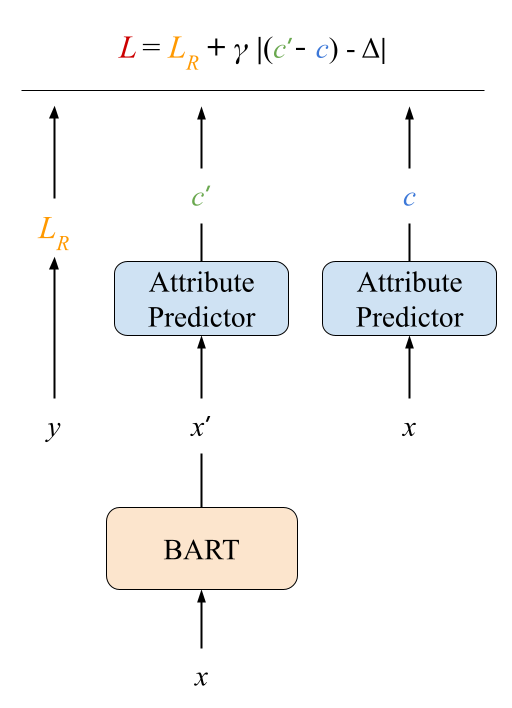
\includegraphics[width=0.9\linewidth]{figs/AC-Architecture.png}
%   \caption{Training diagram for adversarial control of an attribute (\eg speed). We compute the loss as a sum of the negative log likelihood ($L_R$) and the control tuning loss $L_C = \gamma |(c' - c) - \Delta|$.}
%   \label{fig:ac_architecture}
% \end{wrapfigure}

\begin{figure}
    \centering
    \caption{Training diagram for adversarial control of an attribute (\eg speed). We illustrate two approaches to enforce a control constraint via the input $x$: prepending a special token and adding an additional ``speed embedding''. In the latter approach, we add the speed embedding to every layer of BART to ensure information is not lost between encoder/decoder layers. We compute the loss as a weighted sum of the negative log-likelihood ($L_R$) and the control tuning loss $L_C = |(c' - c) - \Delta|$, where $\Delta$ is the desired change in speed. Note that we precompute $c$ to avoid unnecessary inference during training.}
    \label{fig:ac_architecture}
    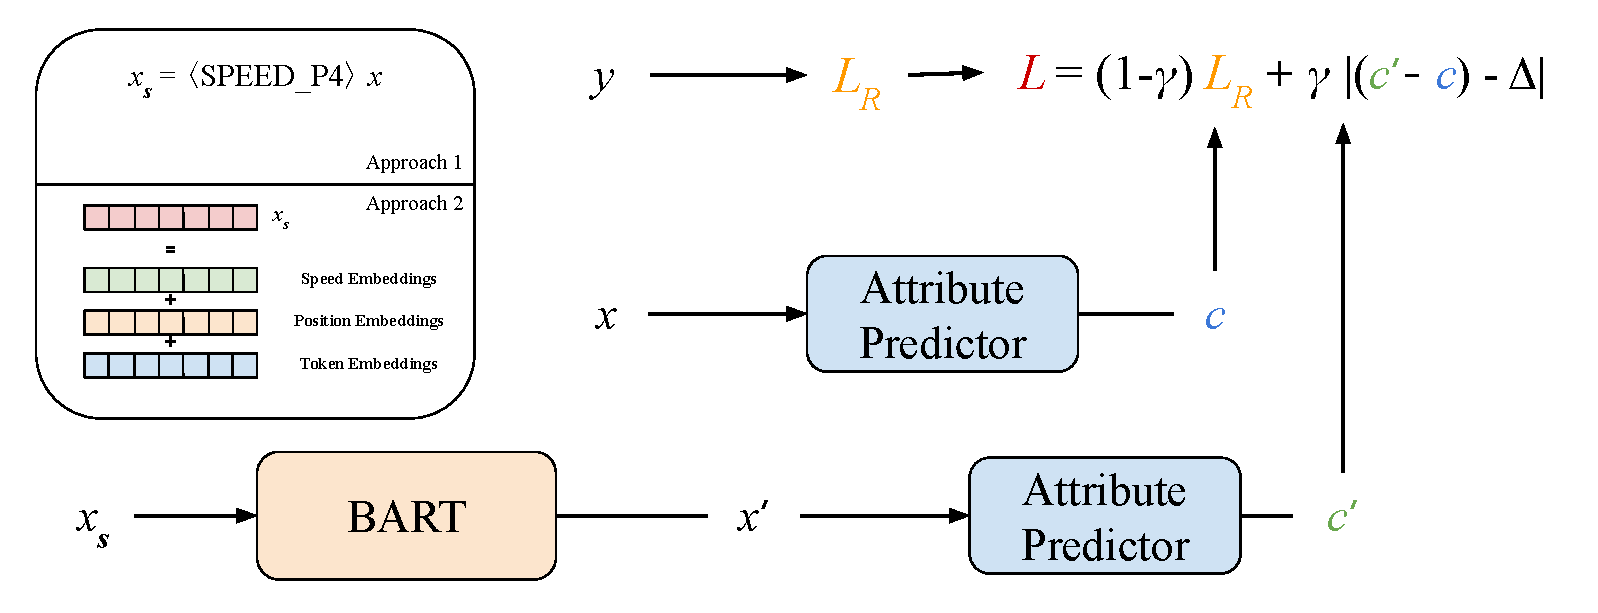
\includegraphics[width=\linewidth]{figs/AC-Architecture-H.pdf}
\end{figure}

In this section, we enforce controls learned by the attribute regressor in~\Cref{subsec:ac_attribute_regressor} into a sequence-to-sequence BART model. The architecture takes in an input sentence $x$ and a desired change in attribute, $\Delta$, generating an output sentence $x'$ that reflects the desired change in the attribute. However, we must modify BART to take $\Delta$ as an input to express the control. We try two methods: prepending a special token and adding a ``speed embedding'' to the token and positional embeddings, as well as in every encoder/decoder layer.

In the former approach, we quantize possible speed values into $2n + 1$ possible bins: $n$ for a positive change in speed, $n$ for a negative change in speed, and $1$ for no change in speed. We convert the bin into a special token containing the strength of change of speed and the direction (\eg ``$\langle$SPEED\_P4$\rangle$'' reflects a change in speed in the fourth highest bin). Each of the $n$ bins covers a range of speeds corresponding to an equal number of samples.

In the latter approach, we add a ``speed embedding'' vector to the token and positional embeddings in BART. The vector is the same size as the token embeddings and is filled with $\Delta$, the desired change in the attribute. We add the embedding vector after every encoder and decoder layer to ensure information is not lost between layers, and then batch normalization is applied.

We use a similar adversarial training paradigm to enable the generator to be controlled by the attribute classifier, illustrated in~\Cref{fig:ac_architecture}. 

\subsection{Training}
\label{subsec:ac_training}

We utilize two losses during training: a reconstruction loss, $L_R$, and a control tuning loss, $L_C$. The reconstruction loss maximizes the log probability of the original sentence, $y_s^*$.

\begin{equation}
    L_{R} = -\frac{1}{N} \sum_{i=1}^{N} \log p(y_s^{*(i)})
\end{equation}

The reconstruction loss teaches the model to mimic the gold-standard samples, preserving content. The control tuning loss enforces a target control and is formulated as follows:

\begin{equation}
    L_{C} = |(\mathcal{A}(x') - \mathcal{A}(x)) - \Delta|
\end{equation}

where $\Delta$ is the desired change in attribute (\eg speed) and $\mathcal{A}(\cdot)$ is the attribute classifier. During training, $x'$ is the first hidden state of the decoder (\ie the representation of the beginning of sequence token), and only the classifier head of the attribute regressor is used to compute the generated sequence's attribute. The final loss is a weighted sum of the two:

\begin{equation}
    L = (1-\gamma) L_R + \gamma L_C
\end{equation}

where $\gamma$ is a hyperparameter to weigh the effect of the control tuning loss and negative log-likelihood. 

\subsection{Experimental Settings}
\label{subsec:ac_experimental}

We train multiple variants of the modified architecture by modifying $\gamma$, the learning rate $\eta$, the attribute classifier architecture (\ie between BART and RoBERTa), and the control method (\ie between the special token and additional embedding methods). 

\textit{\textbf{Perturbation \& $\Delta$-Tolerance Baseline}} We utilize our approach from~\Cref{sec:neural_editor} as a strong baseline. For $\Delta$-Tolerance, we add a $\Delta$ constraint during neighborhood creation and train on the newly formed data. We try $\epsilon = \{0.05, 0.1, 0.2\}$ as tolerance values. For Perturbation, we add the $\Delta$-centered normal distribution to perturb the edit vector during training.

We utilize nucleus sampling to generate sentences with $p=0.8$ and include a repetition penalty \citep{keskar2019ctrl}. We record a few evaluation metrics to test the strength of the control as well as to ensure generations remain similar, lexically and semantically:

\textit{\textbf{METEOR}} We measure the METEOR (Metric for Evaluation of Translation with Explicit ORdering) score \citep{lavie-agarwal-2007-meteor}, essentially the harmonic mean for the test set. While we record BLEU for the previous approach, it will be artificially deflated in this comparison because we are not starting with a prototype. 

\textit{\textbf{BERTScore}} We measure the semantic similarity through the BERTScore \citep{zhang2019bertscore} to ensure that generations remain on topic.

\textit{\textbf{Mean Absolute Error (MAE)}} We record the mean absolute error between the target $\Delta$ and achieved $\Delta$.

\textit{\textbf{MAE From Bounds}} The special token approach for control quantizes speeds, making vanilla MAE an incomplete metric. We also compute the MAE of the generated text's $\Delta$ against the bounds of the respective target bin for speed. More formally, it is represented as 

\begin{equation}
    |\min(l - \Delta, u - \Delta)|
\end{equation}

where $l$ is the lower bound of the bin and $u$ is the upper bound of the bin.

\textit{\textbf{MAE From Center}} Similarly, we compute the MAE of the generated text's $\Delta$ against the mean of the respective target bin. We compute the mean using the $\Delta$s of the training samples instead of directly using $u$ and $l$. 

\subsection{Results}
\label{subsec:ac_results}

% Alter attribute classifier
\begin{table}[]
\centering
\small
\caption{Evaluation metrics for lexical similarity (METEOR \citep{lavie-agarwal-2007-meteor}), semantical similarity (BERTScore \citep{zhang2019bertscore}), and strength of control on $\Delta$, measured with Mean Absolute Error (MAE), MAE from Bounds (MAE-B), and MAE from Center (MAE-C). We compare both the token-based control and the embedding-based control across two different attribute classifier architectures - BART \citep{lewis2019bart}, and RoBERTa \citep{liu2019roberta} - denoted by $\mathcal{A}$. We compare these approaches against the Perturbation \& $\Delta$-Tolerance Baseline from~\Cref{sec:neural_editor}. All of our approaches from this section are trained with $\eta=5e-5$ and $\gamma=0.1$.}
\label{tab:ac_model_variation}

\begin{tabularx}{\linewidth}{@{\extracolsep{\fill}} ccccccc}
\toprule[1.5pt]
                               & $\mathcal{A}$   & \textsc{MAE}    & \textsc{MAE-B} & \textsc{MAE-C} & \textsc{METEOR} & \textsc{BERTScore} \\
\midrule[0.75pt]
Perturb + Tol=0.05             & -               & 0.0721          & -              & -              & 0.5123          & 0.9326 \\
Perturb + Tol=0.1              & -               & 0.0645          & -              & -              & 0.4993          & \textbf{0.9386} \\
Perturb + Tol=0.2              & -               & \textbf{0.0404} & -              & -              & \textbf{0.5391} & 0.9334 \\
\midrule[0.75pt]
\multicolumn{1}{c}{Token}      & BART            & 0.2918          & 0.2136          & 0.2886          & 0.1633          & 0.8710  \\
                               & RoBERTa         & 0.2193          & 0.1405          & 0.2174          & 0.1605          & 0.8749  \\
\midrule[0.75pt]
\multicolumn{1}{c}{Embedding}  & BART            & 0.2819          & -              & -              & 0.1724          & 0.8728  \\
                               & RoBERTa         & 0.2187          & -              & -              & 0.1515          & 0.8728  \\
  \bottomrule[1.5pt]\\
\end{tabularx}
\end{table}

We present the results of our approach in~\Cref{tab:ac_model_variation},~\Cref{tab:ac_lr_variation}, and~\Cref{tab:ac_gamma_variation}, with the former having varied attribute classifier architectures and the latter two having varied learning rates and values of $\gamma$, respectively. The variance across test samples is relatively low for each metric (\eg $0.005$ for BERTScore and $0.03$ for METEOR), so we only report the averaged metric. Our results show that despite the variations of our approach, it fails to outperform our approach from~\Cref{sec:neural_editor}. While lexical and semantical similarity scores are lower than the baseline, this is expected from a larger neural model that is not trained to ``prototype''. However, the metrics for control of speed show that it is difficult for the model to exhibit fine-grained control.

In~\Cref{tab:ac_model_variation}, we find that RoBERTa is significantly stronger than BART in the case of the special token approach, while both are approximately equal in the embedding approach. The decoder layers in BART are likely unnecessary for predicting speed, making RoBERTa more efficient. However, both achieved similar performance on a held-out test set, as mentioned in~\Cref{subsec:ac_attribute_regressor}, implying that RoBERTa developed more robust representations that were transferred during the adversarial training. 

% Alter Learning rate table
\begin{table}[]
\centering
\small
\caption{Evaluation metrics for lexical similarity (METEOR \citep{lavie-agarwal-2007-meteor}), semantical similarity (BERTScore \citep{zhang2019bertscore}), and strength of control on $\Delta$, measured with Mean Absolute Error (MAE), MAE from Bounds (MAE-B), and MAE from Center(MAE-C). We compare the token-based and embedding-based control across three learning rates ($\eta$). We compare these approaches against the Perturbation \& $\Delta$-Tolerance Baseline from~\Cref{sec:neural_editor}. All of our approaches from this section are trained with $\mathcal{A}$ as RoBERTa and $\gamma=0.1$.}
\label{tab:ac_lr_variation}

% 
\begin{tabularx}{\linewidth}{@{\extracolsep{\fill}} ccccccc}
\toprule[1.5pt]
                              & $\eta$           & \textsc{MAE}    & \textsc{MAE-B} & \textsc{MAE-C} & \textsc{METEOR} & \textsc{BERTScore} \\
\midrule[0.75pt]
Perturb + Tol=0.05            & -                & 0.0721          & -              & -              & 0.5123          & 0.9326 \\
Perturb + Tol=0.1             & -                & 0.0645          & -              & -              & 0.4993          & \textbf{0.9386} \\
Perturb + Tol=0.2             & -                & \textbf{0.0404} & -              & -              & \textbf{0.5391} & 0.9334 \\
\midrule[0.75pt]
                              & 1e-5      & 0.3149          & 0.2361         & 0.3111         & 0.1566          & 0.8746  \\
\multicolumn{1}{c}{Token}     & 5e-5      & 0.2193          & 0.1405         & 0.2172         & 0.1605          & 0.8749  \\
                              & 1e-6      & 0.2539          & 0.1754         & 0.2516         & 0.1898          & 0.8710  \\
\midrule[0.75pt]
                              & 1e-5      & 1.7268          & -              & -              & 0.1278          & 0.8721  \\
\multicolumn{1}{c}{Embedding} & 5e-5      & 0.2187          & -              & -              & 0.1515          & 0.8728  \\
                              & 1e-6      & 0.2182          & -              & -              & 0.1724          & 0.8687  \\
  \bottomrule[1.5pt]\\
\end{tabularx}
\end{table}

In~\Cref{tab:ac_lr_variation}, we find an optimal learning rate of $\eta = 5e-5$, which strongly outperforms the other models. Both tables clearly show that the special token-based approach outperforms the embedding-based approach. This result is likely because the special token encodes more information than the uniform embedding, which is confounded with the positional and token embeddings. One exciting avenue for future work is to add the ``control embedding'' to disentangle all three embeddings similarly to \citet{he2020deberta}. 

In~\Cref{tab:ac_gamma_variation}, we vary the value of $\gamma$ across the token-based control. $\gamma=0$ (\ie fine-tuning on our training data) behaves as expected with high lexical and semantic similarity scores, relative to the other values of $\gamma$, but poor control over speed. Empirically, $\gamma = 0.1$ was the strongest approach, balancing control over speed and similarity to the target text. The embedding-based control did not exhibit a significant difference when $\gamma$ was altered; thus, we omitted it from the table.

% Alter gamma table
\begin{table}[]
\centering
\small
\caption{Evaluation metrics for lexical similarity (METEOR \citep{lavie-agarwal-2007-meteor}), semantical similarity (BERTScore \citep{zhang2019bertscore}), and strength of control on $\Delta$, measured with Mean Absolute Error (MAE), MAE from Bounds (MAE-B), and MAE from Center(MAE-C). We compare the token-based control across three different values of $\gamma$. We compare these approaches against the Perturbation \& $\Delta$-Tolerance Baseline from~\Cref{sec:neural_editor}. All of our approaches from this section are trained with $\mathcal{A}$ as RoBERTa and $\eta=5e-5$.}
\label{tab:ac_gamma_variation}

\begin{tabularx}{\linewidth}{@{\extracolsep{\fill}} ccccccc}
\toprule[1.5pt]
                              & $\gamma$           & \textsc{MAE}    & \textsc{MAE-B} & \textsc{MAE-C} & \textsc{METEOR} & \textsc{BERTScore} \\
\midrule[0.75pt]
Perturb + Tol=0.05            & -                & 0.0721          & -              & -              & 0.5123          & 0.9326 \\
Perturb + Tol=0.1             & -                & 0.0645          & -              & -              & 0.4993          & \textbf{0.9386} \\
Perturb + Tol=0.2             & -                & \textbf{0.0404} & -              & -              & \textbf{0.5391} & 0.9334 \\
\midrule[0.75pt]
                              & 0.0              & 0.5051          & 0.4282         & 0.4889         & 0.1724          & 0.8877  \\
\multicolumn{1}{c}{Token}     & 0.1              & 0.2193          & 0.1405         & 0.2172         & 0.1605          & 0.8749  \\
                              & 0.2              & 0.2517          & 0.1730         & 0.2492         & 0.1655          & 0.8710  \\
                              & 0.5              & 0.3304          & 0.2501         & 0.3251         & 0.1446          & 0.8746  \\
  \bottomrule[1.5pt]\\
\end{tabularx}
\end{table}

\Cref{tab:ac_example} shows the generations of the baselines of the previous approach (\S\ref{sec:neural_editor}) and $\gamma$-variants of the adversarial training approach. We find that while all generations are generally fluent and on topic, the change in speed of the baseline approach, $\gamma=0.1$, and $\gamma=0.2$ are more positive than the other approaches, as they tend to cover more content in a shorter time frame. However, it is interesting that the generations of $\gamma=0.0$ are similar to, if not the same as, generations from models with the control tuning loss. We also notice that this approach tends to hallucinate some details. For example, for the input ``He went above and beyond in providing us excellent customer service and was extremely courteous friendly and kind,'' the model generates ``The service was great, the gentleman who helped us was very friendly and helpful. \textit{He made sure we were happy with our purchase},'' incorrectly implying the reviewer made a purchase. However, this is a common problem in existing generation models \citep{ji2022survey}, and we leave it to future work to explore this issue in depth.

  \begin{table}[htb]
  \small
  \centering
  \caption{The previous section's approach (Perturbation + Tol=0.2) along with variants of our adversarial training approach. Neighborhood creation models are listed as ``Tol=$\epsilon$'' where $\epsilon$ is the tolerance. The adversarially-trained models are all trained with the Token-based method, RoBERTa as $\mathcal{A}$, and $\eta=5e-5$ as they are empirically the best settings. We vary the value of $\gamma$ to test the impact of the control tuning loss. The models are fed the input (\ie \textbf{Original}) with a target $\Delta=0.5$ and either generate by applying an ``edit vector'' to the latent representation of the input or through nucleus sampling with $p=0.8$.}
  \label{tab:ac_example} 
  \begin{tabularx}{\linewidth}{@{}>{\raggedright\arraybackslash}X@{}}
   \toprule[1.5pt]
  \textsc{Model} \& \textsc{Generated Text}\\
  \midrule[0.75pt]
  \textsc{Example 1:}\\
  \textbf{Original}: He went above and beyond in providing us excellent customer service and was extremely courteous friendly and kind.  \\
  \textbf{Perturbation + Tol=0.2}: He was knowledgable, courteous, and went provided excellent customer service.\\
  \textbf{Ours ($\gamma=0.0$)}: The service was great. The gentleman who helped us was very friendly and helpful, but not pushy at all.\\
  \textbf{Ours ($\gamma=0.1$)}:  The service was great, the gentleman who helped us was very friendly and helpful. He made sure we were happy with our purchase!\\
  \textbf{Ours ($\gamma=0.2$)}:  The service was prompt and friendly and the food delicious.  Also cheap as hell.\\
  \textbf{Ours ($\gamma=0.5$)}: He was very friendly and helpful. He made our experience a great one! Thank you for being such an amazing customer service!! \\
  \addlinespace[0.5em]
  \textsc{Example 2:}\\
  \textbf{Original}: The staff is very professional and friendly \& environment is clean.  \\
  \textbf{Perturbation + Tol=0.2}: Friendly staff and clean environment.\\
  \textbf{Ours ($\gamma=0.0$)}: The staff is very friendly and helpful. \\
  \textbf{Ours ($\gamma=0.1$)}: The staff is very friendly and helpful. \\
  \textbf{Ours ($\gamma=0.2$)}:  The staff is friendly.\\
  \textbf{Ours ($\gamma=0.5$)}:  The staff is very friendly and professional.  The place is clean, well kept and the environment was nice as well!\\
  \bottomrule[1.5pt]\\
  \end{tabularx}
  \vspace{-10px}
  \end{table}

While the approach was relatively successful in some settings, fine-tuning the entire BART model may be unnecessarily expensive and degrade generation quality. \citet{li2021prefix} propose a lightweight alternative that optimizes the prefix, a relatively small, task-specific, continuous vector prepended to the input. By learning a small fraction of the parameters of the entire model, prefix-tuning capitalizes on extensive pretraining while outperforming other baselines in task-specific settings. Initial experiments have shown some promise, but we want to continue exploring this direction for lightweight, controllable text generation techniques. We also leave it to future work to discover methods for multiple constraints and to empirically investigate existing formulations that allow for more than one control.

In this section, we propose an adversarial training framework to control the speed of generated text and show that our approach exhibits decent control over speed. We propose a few avenues to improve this exploratory work which we plan to continue investigating.
